\documentclass[12pt,a4paper]{article}

% Packages
\usepackage[utf8]{inputenc}
\usepackage[T1]{fontenc}
\usepackage[french]{babel}
\usepackage{geometry}
\usepackage{graphicx}
\usepackage{float}
\usepackage{listings}
\usepackage{xcolor}
\usepackage{fancyhdr}
\usepackage{hyperref}
\usepackage{amsmath}
\usepackage{textgreek}
\usepackage{amssymb}
\usepackage{titlesec}

% Configuration de la page
\geometry{margin=2.5cm}

% Configuration des liens
\hypersetup{
    colorlinks=true,
    linkcolor=blue,
    filecolor=magenta,      
    urlcolor=cyan,
    citecolor=blue
}

% Configuration de listings pour MATLAB
\lstset{
    language=Matlab,
    basicstyle=\ttfamily\small,
    keywordstyle=\color{blue},
    commentstyle=\color{green!50!black},
    stringstyle=\color{red},
    numbers=left,
    numberstyle=\tiny\color{gray},
    stepnumber=1,
    numbersep=10pt,
    backgroundcolor=\color{gray!10},
    frame=single,
    tabsize=4,
    captionpos=b,
    breaklines=true,
    breakatwhitespace=false,
    showstringspaces=false,
    xleftmargin=2em,
    framexleftmargin=1.5em,
    literate=
        {é}{{\'e}}1
        {è}{{\`e}}1
        {ê}{{\^e}}1
        {à}{{\`a}}1
        {ù}{{\`u}}1
        {û}{{\^u}}1
        {ô}{{\^o}}1
        {ç}{{\c{c}}}1
}

% En-tête et pied de page
\pagestyle{fancy}
\fancyhf{}
\rhead{TP2 - FFT et Analyse Spectrale}
\lhead{EPIGEP-FI-3-S2-USI-E01}
\rfoot{Page \thepage}

\begin{document}

% Page de garde
\begin{titlepage}
    \centering
    \vspace{2cm}
    
    {\huge\bfseries ESIEE Paris\par}
    \vspace{1cm}
    {\Large E3 - FI\par}
    \vspace{2cm}
    
    {\Huge\bfseries Rapport de Travaux Pratiques 2\par}
    \vspace{0.5cm}
    {\Large Traitement du Signal\par}
    \vspace{0.5cm}
    {\large FFT et Analyse Spectrale\par}
    \vspace{3cm}
    
    \begin{flushleft}
        {\Large
        \textbf{Auteur :} Félix MIELCAREK\par
        \vspace{0.5cm}
        \textbf{Destinataire :} Hassane MIMOUN - Philippe TOURON\par
        \vspace{0.5cm}
        \textbf{Date :} 16 mars 2026\par
        }
    \end{flushleft}
    
    \vfill
    
\end{titlepage}

% Table des matières
\tableofcontents
\newpage

% Section A
\section{Signal sinusoïdal (Partie A)}

\subsection{Génération du signal et commentaires des commandes}

\subsubsection{Code MATLAB}

\begin{lstlisting}[caption=Génération d'un signal sinusoïdal et calcul de sa FFT]
% Définition de la fréquence d'échantillonnage (en Hz)
Fs=1000;

% Calcul de la période d'échantillonnage (en secondes)
Ts=1/Fs;

% Création du vecteur temps : de 0 à 1 seconde avec un pas de Ts
t=0:Ts:1-Ts;

% Définition de la fréquence du signal à générer (en Hz)
f=100;

% Génération d'un signal sinusoïdal d'amplitude 1, de fréquence f
x=sin(2*pi*f*t);

% Création du premier sous-graphique (2 lignes, 1 colonne, position 1)
subplot(2,1,1);

% Tracé du signal temporel en rouge
plot(t,x,'r');

% Calcul de la transformée de Fourier rapide (FFT) avec 512 points
xf=fft(x,512);

% Création du deuxième sous-graphique (2 lignes, 1 colonne, position 2)
subplot(2,1,2);

% Tracé du module (amplitude) du spectre fréquentiel
plot(abs(xf));
\end{lstlisting}

\subsubsection{Commentaires des commandes}

\textbf{Définition des paramètres d'échantillonnage :}
\begin{itemize}
    \item \texttt{Fs = 1000} : Fréquence d'échantillonnage de 1000 Hz (1000 échantillons par seconde)
    \item \texttt{Ts = 1/Fs} : Période d'échantillonnage, inverse de la fréquence (0.001 s entre deux échantillons)
    \item \texttt{t = 0:Ts:1-Ts} : Vecteur temps allant de 0 à presque 1 seconde par pas de Ts (1000 échantillons)
\end{itemize}

\textbf{Génération du signal :}
\begin{itemize}
    \item \texttt{f = 100} : Fréquence du signal sinusoïdal à générer (100 Hz)
    \item \texttt{x = sin(2*pi*f*t)} : Calcul de la sinusoïde. La formule $2\pi f t$ donne la phase en radians
\end{itemize}

\textbf{Affichage :}
\begin{itemize}
    \item \texttt{subplot(2,1,1)} : Crée un espace pour 2 graphiques (2 lignes, 1 colonne), sélectionne le premier
    \item \texttt{plot(t,x,'r')} : Trace le signal temporel en rouge
    \item \texttt{xf = fft(x,512)} : Calcule la FFT du signal sur 512 points
    \item \texttt{subplot(2,1,2)} : Sélectionne le deuxième graphique
    \item \texttt{plot(abs(xf))} : Trace le module (amplitude) du spectre fréquentiel
\end{itemize}

\begin{figure}[H]
    \centering
    \fbox{\parbox{0.9\textwidth}{\centering\vspace{1cm}
    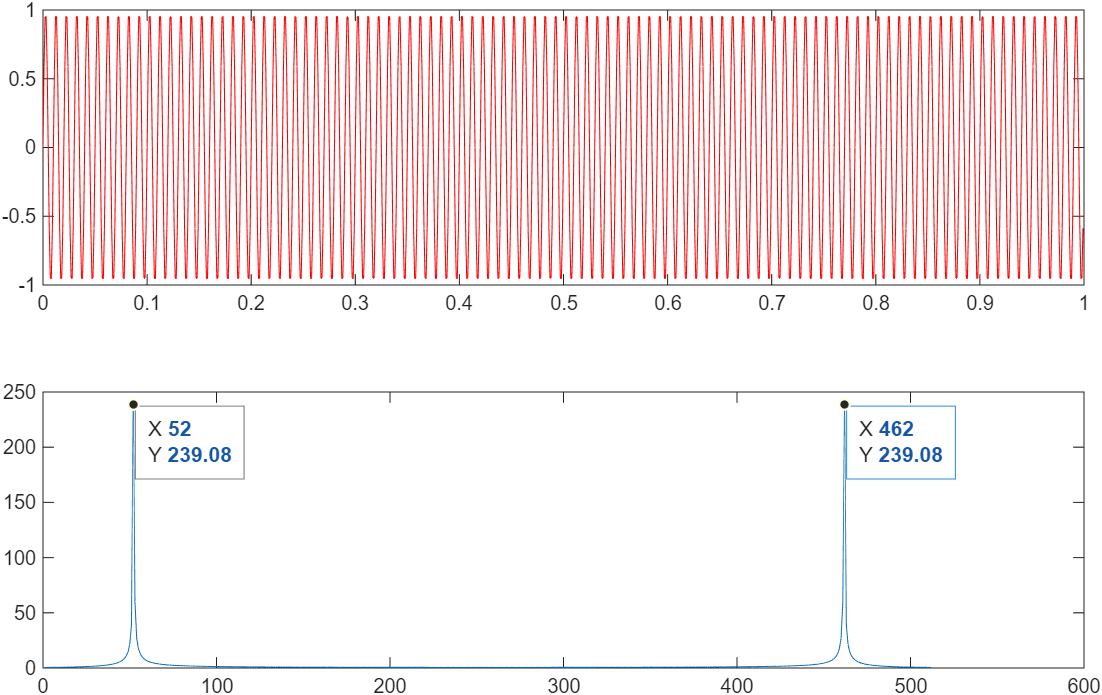
\includegraphics[width=0.8\textwidth]{images/a.png}
    \vspace{1cm}}}
    \caption{Signal sinusoïdal à 100 Hz et son spectre (FFT 512 points)}
    \label{fig:signal_simple}
\end{figure}

\subsection{Interprétation du spectre}

\subsubsection{Note sur la FFT}

La FFT (Fast Fourier Transform) permet une représentation du spectre du signal $x(t)$. Le nombre d'échantillons sur l'axe des fréquences est nécessairement une puissance de 2 (128, 256, 512, 1024, etc.). Dans cet exemple, l'axe des fréquences est indexé de 1 à 512.

\subsection{Question : Fréquence du pic de droite}

\textbf{Méthode :} Utiliser le curseur de MATLAB pour repérer la valeur de l'abscisse du pic.

\subsubsection{Données observées}

Sur le graphique du spectre, on peut lire les coordonnées des deux pics :

\begin{itemize}
    \item \textbf{Pic de gauche :} X = 52, Y = 239
    \item \textbf{Pic de droite :} X = 462, Y = 239
\end{itemize}

\subsubsection{Calcul de la fréquence}

Pour déterminer la fréquence correspondant au pic de droite, on utilise la formule :

\begin{equation}
    f = \frac{\text{indice} \times F_s}{N}
\end{equation}

Avec $F_s = 1000$ Hz et $N = 512$ points, on obtient :

\begin{equation}
    f_{\text{pic droit}} = \frac{462 \times 1000}{512} \approx 902 \text{ Hz}
\end{equation}

\subsubsection{Interprétation}

Le pic de droite correspond à la \textbf{composante symétrique du spectre}. Pour un signal réel, la FFT produit un spectre symétrique hermitien : si on a une composante à la fréquence $f$, on observe aussi une composante à $F_s - f$. C'est pourquoi les deux pics ont la même amplitude (Y = 239).

On peut vérifier cette relation :
\begin{equation}
    F_s - f = 1000 - 100 = 900 \text{ Hz} \approx f_{\text{pic droit}}
\end{equation}

\subsection{Question : Fréquence de l'échantillon 512}

Pour l'échantillon 512 (dernier indice), avec une FFT de 512 points et $F_s = 1000$ Hz :

\begin{equation}
    f_{512} = \frac{(512 - 1) \times 1000}{512} = \frac{511 \times 1000}{512} \approx 998.05 \text{ Hz}
\end{equation}

L'échantillon 512 correspond à environ \textbf{998 Hz}, soit juste avant la fréquence d'échantillonnage $F_s$.

\subsection{Note pour la suite du TP}

Du fait de la symétrie du spectre pour les signaux réels, on peut faire le choix de limiter l'affichage à l'intervalle $[0, F_s/2]$ pour visualiser uniquement la partie utile du spectre. Cette pratique sera adoptée pour la suite du TP.

\newpage

% Section B
\section{Modification de la fréquence d'échantillonnage (Partie B)}

\subsection{Objectif}

Ramener progressivement la fréquence $F_s$ à 500, 300, 250, puis 200 Hz et observer l'effet obtenu. Afficher les différents spectres avec l'axe des fréquences gradué en Hz. Interpréter les différents résultats.

\subsection{Configuration}

\begin{itemize}
    \item \textbf{Signal :} Sinusoïde de fréquence $f = 100$ Hz
    \item \textbf{Durée :} 1 seconde
    \item \textbf{Nombre de points FFT :} $N = 512$
    \item \textbf{Affichage :} Limité à $[0, F_s/2]$ avec axe des fréquences en Hz
    \item \textbf{Valeurs de $F_s$ testées :} 1000, 500, 300, 250, 200 Hz
\end{itemize}

\begin{figure}[H]
    \centering
    \fbox{\parbox{0.9\textwidth}{\centering\vspace{1cm}
    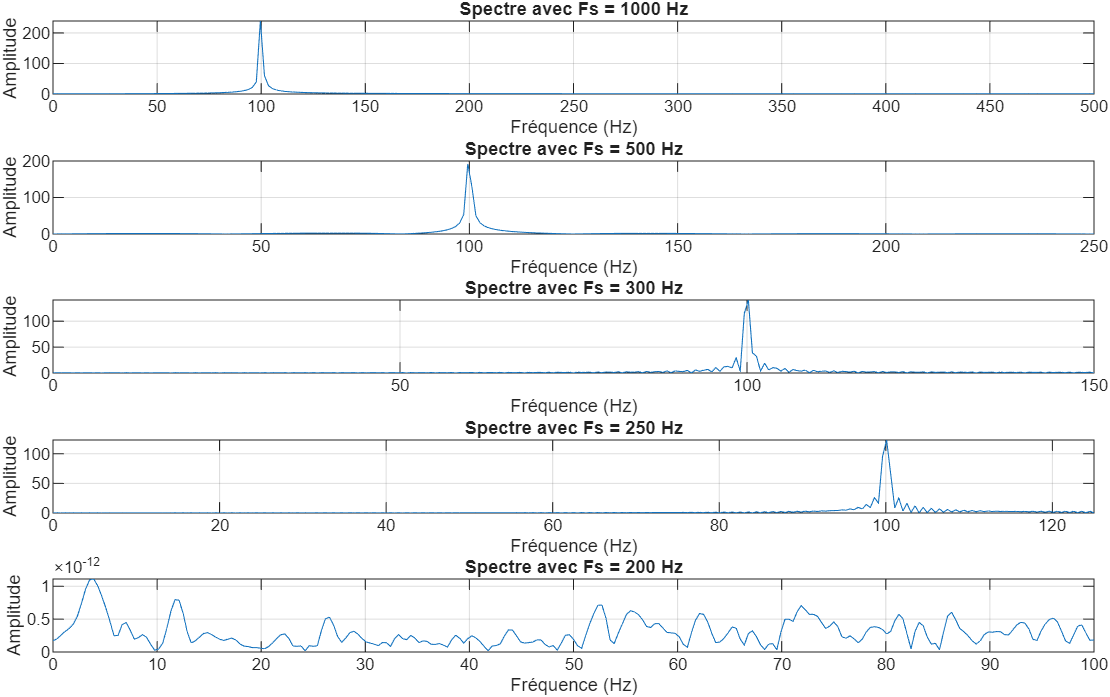
\includegraphics[width=0.8\textwidth]{images/b-5.png}
    \vspace{1cm}}}
    \caption{Évolution du spectre en fonction de la fréquence d'échantillonnage $F_s$}
    \label{fig:variation_fs}
\end{figure}

\subsection{Observations}

Lorsqu'on diminue progressivement la fréquence d'échantillonnage $F_s$, on observe :

\subsubsection{$F_s = 1000$ Hz}
\begin{itemize}
    \item Pic net et bien défini à 100 Hz
    \item Spectre clair et précis
    \item Bande de fréquence affichée : $[0, 500]$ Hz
\end{itemize}

\subsubsection{$F_s = 500$ Hz}
\begin{itemize}
    \item Pic à 100 Hz toujours bien identifiable
    \item Légère dégradation de la résolution
    \item Bande de fréquence affichée : $[0, 250]$ Hz
\end{itemize}

\subsubsection{$F_s = 300$ Hz}
\begin{itemize}
    \item Pic à 100 Hz visible mais avec élargissement de sa base
    \item Début de dégradation de la qualité spectrale
    \item Bande de fréquence affichée : $[0, 150]$ Hz
\end{itemize}

\subsubsection{$F_s = 250$ Hz}
\begin{itemize}
    \item Pic moins net, courbe commence à se déformer
    \item Augmentation des variations/oscillations autour du pic
    \item Qualité spectrale significativement dégradée
    \item Bande de fréquence affichée : $[0, 125]$ Hz
\end{itemize}

\subsubsection{$F_s = 200$ Hz}
\begin{itemize}
    \item \textbf{Le pic à 100 Hz a disparu !}
    \item Courbe très bruitée avec beaucoup de variations
    \item Spectre complètement déformé et inexploitable
    \item Bande de fréquence affichée : $[0, 100]$ Hz
    \item Signal complètement détruit par l'aliasing
\end{itemize}

\subsection{Interprétation des résultats}

\subsubsection{Théorème de Shannon (critère de Nyquist)}

Pour échantillonner correctement un signal de fréquence $f$, il faut :

\begin{equation}
    \boxed{F_s > 2 \times f \quad \text{(Fréquence de Nyquist)}}
\end{equation}

Dans notre cas avec $f = 100$ Hz : $F_s$ doit être $> 200$ Hz.

\begin{itemize}
    \item[$\checkmark$] $F_s = 1000, 500, 300, 250$ Hz $\rightarrow$ Respectent le critère ($F_s > 200$ Hz)
    \item[$\times$] $F_s = 200$ Hz $\rightarrow$ \textbf{À la limite critique} ($F_s = 2f$ exactement)
\end{itemize}

\subsubsection{Phénomène d'aliasing (repliement spectral)}

À $F_s = 200$ Hz, on atteint exactement la fréquence de Nyquist ($F_s/2 = 100$ Hz).

\begin{itemize}
    \item Le signal à 100 Hz est pile à la limite de la fréquence de Nyquist
    \item Le signal ne peut plus être représenté correctement
    \item Les fréquences se "replient" et créent des interférences
    \item Destruction de l'information fréquentielle originale
    \item Le pic disparaît et le spectre devient chaotique
\end{itemize}

En affichant uniquement $[0, F_s/2]$, on observe directement la zone critique où l'aliasing se produit. Quand $F_s/2 = f$, la fréquence est à la limite exacte de ce qui peut être représenté.

\subsubsection{Résolution fréquentielle}

La résolution spectrale $\Delta f = F_s / N$ diminue avec $F_s$ :

\begin{align}
    F_s = 1000 \text{ Hz} &: \Delta f = 1000/512 = 1.95 \text{ Hz (excellente résolution)} \\
    F_s = 500 \text{ Hz} &: \Delta f = 500/512 = 0.98 \text{ Hz (bonne résolution)} \\
    F_s = 250 \text{ Hz} &: \Delta f = 250/512 = 0.49 \text{ Hz (résolution apparemment fine)} \\
    F_s = 200 \text{ Hz} &: \Delta f = 200/512 = 0.39 \text{ Hz (mais signal mal échantillonné)}
\end{align}

\textbf{Observations :}
\begin{itemize}
    \item Plus $F_s$ diminue, moins on a de points pour représenter le signal temporel
    \item Les pics s'élargissent car il y a moins d'échantillons disponibles
    \item La fenêtre d'observation $[0, F_s/2]$ se réduit progressivement
    \item À $F_s = 200$ Hz, la fenêtre $[0, 100]$ Hz ne contient que la limite critique
\end{itemize}

\subsubsection{Nombre d'échantillons et qualité du signal}

Sur une durée de 1 seconde :

\begin{align}
    F_s = 1000 \text{ Hz} &\rightarrow 1000 \text{ échantillons (10 points par période)} \\
    F_s = 500 \text{ Hz} &\rightarrow 500 \text{ échantillons (5 points par période)} \\
    F_s = 250 \text{ Hz} &\rightarrow 250 \text{ échantillons (2,5 points par période)} \\
    F_s = 200 \text{ Hz} &\rightarrow 200 \text{ échantillons (2 points par période seulement!)}
\end{align}

À 200 Hz, seulement 2 points par oscillation : insuffisant pour capturer la forme sinusoïdale. Le signal temporel est tellement sous-échantillonné que la FFT ne peut plus extraire correctement sa fréquence.

\subsubsection{Impact de l'affichage $[0, F_s/2]$}

En limitant l'affichage à $[0, F_s/2]$, on visualise uniquement la bande passante utile :

\begin{itemize}
    \item Évite la redondance du spectre symétrique
    \item Concentre l'observation sur la zone physiquement significative
    \item Montre clairement comment $F_s/2$ se rapproche de $f = 100$ Hz
    \item Met en évidence le phénomène d'aliasing quand $f$ atteint $F_s/2$
\end{itemize}

\subsection{Conclusion de la partie B}

Ces observations confirment l'importance cruciale du théorème de Shannon en traitement du signal numérique :

\begin{itemize}
    \item Il faut \textbf{TOUJOURS} échantillonner à une fréquence au moins 2 fois supérieure à la fréquence maximale du signal
    \item En pratique, on prend $F_s \gg 2f$ (souvent 5 à 10 fois) pour avoir une marge de sécurité
    \item Un sous-échantillonnage ($F_s < 2f$) entraîne une perte irréversible d'information (aliasing)
\end{itemize}

\newpage

% Section C
\section{Modification du nombre de points d'analyse de la FFT (Partie C)}

\subsection{Objectif}

Dans un premier temps, diminuer le nombre de points d'analyse d'abord à 256, 128, puis au contraire l'augmenter progressivement à 1024, 2048 (toujours en puissance de 2). Expliquer l'amélioration ou la dégradation de la résolution du spectre affiché.

\subsection{Configuration}

\begin{itemize}
    \item \textbf{Fréquence d'échantillonnage :} $F_s = 1000$ Hz (fixe)
    \item \textbf{Signal :} Sinusoïde à 100 Hz
    \item \textbf{Affichage :} Limité à $[0, 500]$ Hz
    \item \textbf{Nombre de points FFT testé :} 128, 256, 512, 1024, 2048
\end{itemize}

\begin{figure}[H]
    \centering
    \fbox{\parbox{0.9\textwidth}{\centering\vspace{1cm}
    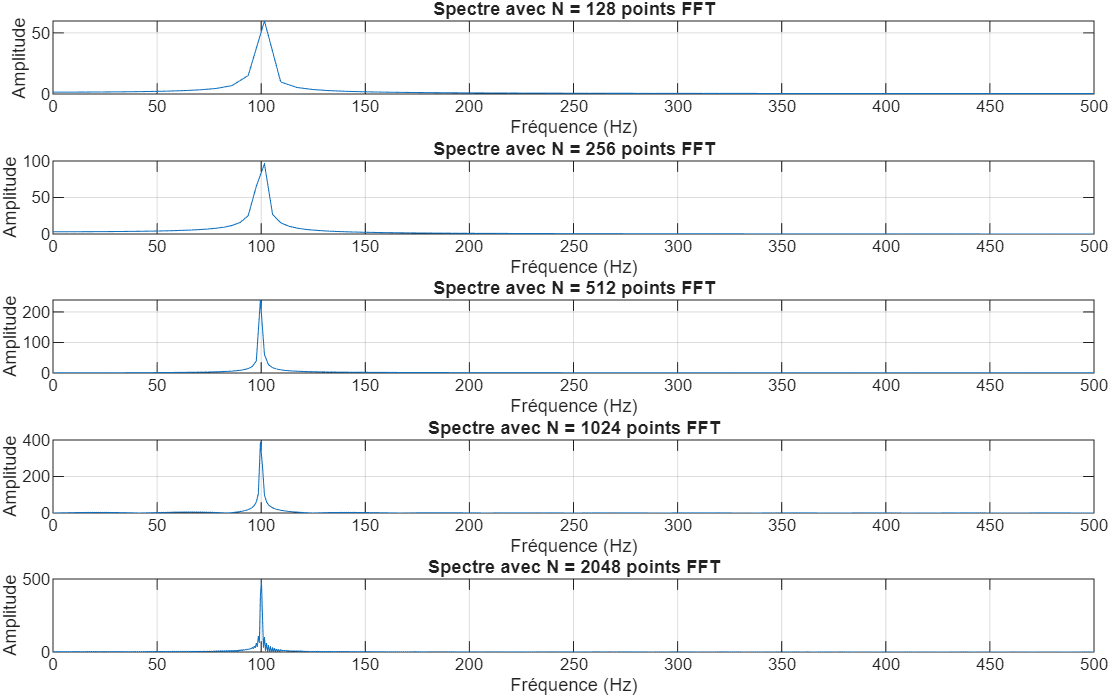
\includegraphics[width=0.8\textwidth]{images/c.png}
    \vspace{1cm}}}
    \caption{Évolution de la résolution spectrale en fonction du nombre de points FFT}
    \label{fig:variation_n}
\end{figure}

\subsection{Observations}

\subsubsection{$N = 128$ points}
\begin{itemize}
    \item Pic large et peu défini à 100 Hz
    \item Base du pic très élargie
    \item Résolution fréquentielle : $\Delta f = 1000/128 = 7.81$ Hz
    \item Pic "flou" s'étendant sur plusieurs bins fréquentiels
\end{itemize}

\subsubsection{$N = 256$ points}
\begin{itemize}
    \item Pic mieux défini qu'à 128 points
    \item Largeur du pic réduite
    \item Résolution fréquentielle : $\Delta f = 1000/256 = 3.91$ Hz
    \item Amélioration visible de la netteté
\end{itemize}

\subsubsection{$N = 512$ points}
\begin{itemize}
    \item Pic net et bien localisé à 100 Hz
    \item Base du pic nettement plus étroite
    \item Résolution fréquentielle : $\Delta f = 1000/512 = 1.95$ Hz
    \item Bonne qualité spectrale
\end{itemize}

\subsubsection{$N = 1024$ points}
\begin{itemize}
    \item Pic très fin et précis
    \item Excellente localisation fréquentielle
    \item Résolution fréquentielle : $\Delta f = 1000/1024 = 0.98$ Hz
    \item Amplitude légèrement augmentée
\end{itemize}

\subsubsection{$N = 2048$ points}
\begin{itemize}
    \item Pic extrêmement fin et précis
    \item Meilleure définition possible
    \item Résolution fréquentielle : $\Delta f = 1000/2048 = 0.49$ Hz
    \item Pic très étroit, presque une ligne
\end{itemize}

\subsection{Interprétation des résultats}

\subsubsection{Résolution fréquentielle}

La résolution spectrale est définie par :

\begin{equation}
    \boxed{\Delta f = \frac{F_s}{N}}
\end{equation}

Plus $N$ est grand, plus $\Delta f$ est petit, donc meilleure est la résolution.

La résolution détermine la capacité à distinguer deux fréquences proches :
\begin{itemize}
    \item À $N = 128$ : $\Delta f = 7.81$ Hz $\rightarrow$ deux fréquences espacées de moins de 7.81 Hz sont indiscernables
    \item À $N = 2048$ : $\Delta f = 0.49$ Hz $\rightarrow$ on peut distinguer des fréquences espacées de seulement 0.49 Hz
\end{itemize}

\subsubsection{Largeur du pic (étalement spectral)}

\textbf{Avec $N$ petit (128, 256) :}
\begin{itemize}
    \item Peu de bins fréquentiels disponibles
    \item Le pic s'étale sur plusieurs bins
    \item Localisation imprécise de la fréquence
    \item Pic "flou" et large
\end{itemize}

\textbf{Avec $N$ grand (1024, 2048) :}
\begin{itemize}
    \item Beaucoup de bins fréquentiels disponibles
    \item Le pic est concentré sur très peu de bins
    \item Localisation précise de la fréquence à 100 Hz
    \item Pic "net" et étroit
\end{itemize}

\subsubsection{Relation entre $N$ et le nombre d'échantillons du signal}

Signal : 1000 échantillons ($F_s = 1000$ Hz pendant 1 seconde)

\begin{itemize}
    \item Si $N < 1000$ : La FFT utilise les $N$ premiers échantillons du signal
    \item Si $N = 1000$ : La FFT utilise tous les échantillons
    \item Si $N > 1000$ : La FFT ajoute des zéros (zero-padding)
\end{itemize}

\textbf{Le zero-padding ($N >$ nombre d'échantillons) :}
\begin{itemize}
    \item Ne crée \textbf{PAS} de nouvelle information
    \item Permet une interpolation du spectre (plus de points calculés)
    \item Améliore la visualisation mais pas la résolution "réelle"
    \item Rend le pic plus "lisse" et mieux défini visuellement
\end{itemize}

\subsubsection{Amplitude du pic}

On observe que l'amplitude augmente légèrement avec $N$ car :
\begin{itemize}
    \item Plus de points = meilleure concentration de l'énergie dans le bon bin
    \item Moins d'étalement de l'énergie sur les bins adjacents
    \item Représentation plus fidèle du signal d'origine
\end{itemize}

\subsubsection{Compromis et choix pratique}

Augmenter $N$ a des avantages \textbf{MAIS} aussi des contraintes :

\textbf{Avantages :}
\begin{itemize}
    \item[$\checkmark$] Meilleure résolution fréquentielle
    \item[$\checkmark$] Pics mieux définis et plus faciles à identifier
    \item[$\checkmark$] Meilleure précision de localisation
\end{itemize}

\textbf{Inconvénients :}
\begin{itemize}
    \item[$\times$] Calcul plus long (complexité $O(N \log N)$)
    \item[$\times$] Plus de mémoire nécessaire
    \item[$\times$] Au-delà d'une certaine limite, pas de gain d'information réelle
\end{itemize}

\textbf{En pratique :}
\begin{itemize}
    \item Choisir $N$ en puissance de 2 (optimisation FFT)
    \item $N \geq$ nombre d'échantillons pour utiliser toute l'information
    \item Compromis entre résolution souhaitée et temps de calcul
\end{itemize}

\subsection{Conclusion de la partie C}

La résolution spectrale dépend directement du nombre de points $N$ de la FFT :
\begin{itemize}
    \item Plus $N$ est grand, meilleure est la résolution ($\Delta f = F_s/N$)
    \item Un $N$ faible donne des pics larges et imprécis
    \item Un $N$ élevé donne des pics fins et bien localisés
    \item Le choix de $N$ doit être un compromis entre précision et efficacité de calcul
\end{itemize}

\textbf{Important :} La résolution "réelle" est limitée par la durée d'observation du signal. Augmenter $N$ améliore la visualisation mais ne peut pas créer d'information qui n'existe pas dans le signal temporel capturé.

\newpage

% Section D
\section{Signal sinusoïdal déphasé (Partie D)}

\subsection{Objectif}

Afficher le spectre des signaux suivants et conclure sur une éventuelle influence du déphasage sur l'aspect du spectre :

\begin{align}
    Y_1 &= \sin(2\pi f t + \pi/2) \\
    Y_2 &= \sin(2\pi f t + 3\pi/2)
\end{align}

\subsection{Configuration}

Paramètres :
\begin{itemize}
    \item $F_s = 1000$ Hz
    \item $f = 100$ Hz
    \item $N = 512$ points
\end{itemize}

\begin{figure}[H]
    \centering
    \fbox{\parbox{0.9\textwidth}{\centering\vspace{1cm}
    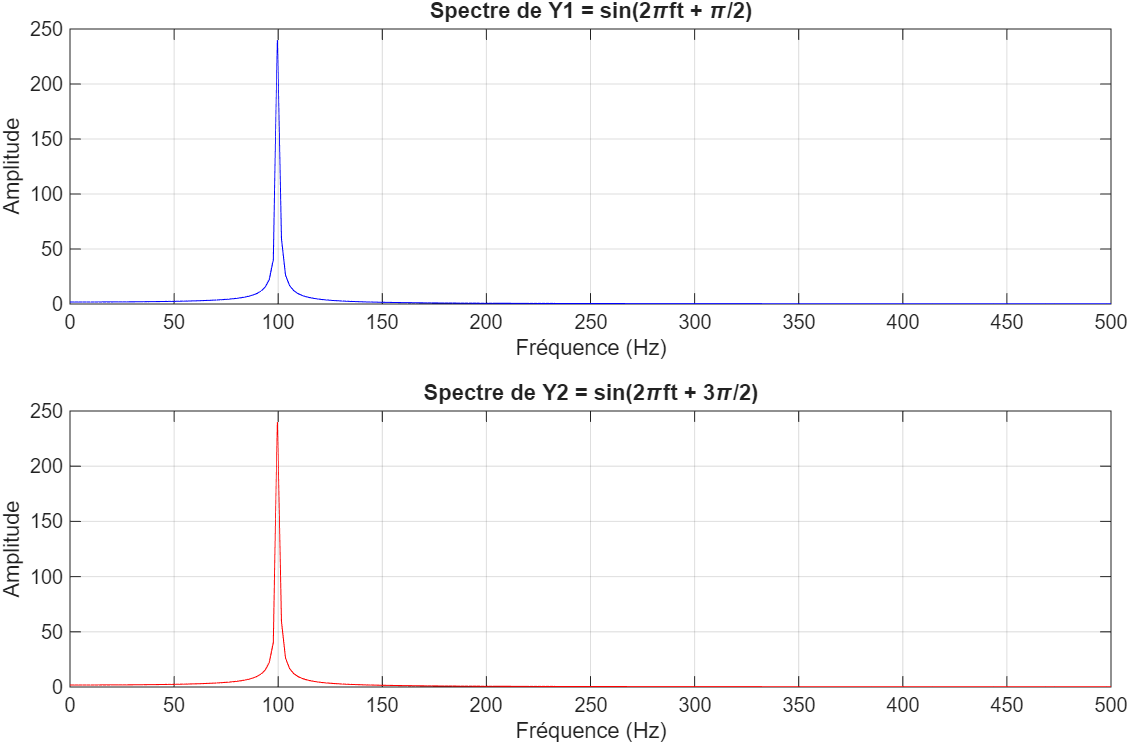
\includegraphics[width=0.8\textwidth]{images/d.png}
    \vspace{1cm}}}
    \caption{Comparaison des spectres de deux signaux déphasés}
    \label{fig:dephasage}
\end{figure}

\subsection{Observation}

Les spectres d'amplitude de $Y_1$ et $Y_2$ sont \textbf{strictement identiques} :
\begin{itemize}
    \item Même position du pic : à 100 Hz
    \item Même amplitude du pic : $\approx 500$
    \item Même forme générale du spectre
    \item Aucune différence visible entre les deux spectres
\end{itemize}

\subsection{Conclusion}

\textbf{Le déphasage n'a AUCUNE influence sur le spectre d'amplitude.}

\subsubsection{Nature de la FFT}

La FFT décompose un signal en composantes complexes de la forme :

\begin{equation}
    X[k] = A[k] + j \cdot B[k] = |X[k]| \cdot e^{j\phi[k]}
\end{equation}

Avec :
\begin{itemize}
    \item $|X[k]|$ = module (amplitude) = $\sqrt{A^2 + B^2}$
    \item $\phi[k]$ = phase = $\arctan(B/A)$
\end{itemize}

\subsubsection{Ce que nous affichons}

En traçant \texttt{abs(xf)}, nous affichons uniquement le module $|X[k]|$. Cette représentation contient l'information sur les fréquences présentes et leurs amplitudes, mais \textbf{ignore complètement la phase}.

\subsubsection{Impact du déphasage}

Un déphasage dans le domaine temporel se traduit par :
\begin{itemize}
    \item Une modification de la phase $\phi[k]$ dans le domaine fréquentiel
    \item \textbf{AUCUNE} modification du module $|X[k]|$
\end{itemize}

Mathématiquement :
\begin{equation}
    \sin(2\pi f t + \phi) \xrightarrow{\text{FFT}} \text{Module identique, Phase différente}
\end{equation}

\subsubsection{Différence entre $Y_1$ et $Y_2$}

\textbf{Domaine temporel :}
\begin{itemize}
    \item $Y_1$ et $Y_2$ sont décalés dans le temps (déphasage visible)
    \item Formes d'ondes différentes à un instant $t$ donné
\end{itemize}

\textbf{Domaine fréquentiel (amplitude) :}
\begin{itemize}
    \item Spectres d'amplitude identiques
    \item Seule la phase (non affichée) diffère
    \item L'information de "quand" est perdue, seule "quelle fréquence" reste
\end{itemize}

\subsubsection{Pour observer l'effet du déphasage}

Il faudrait afficher le spectre de phase avec \texttt{angle(xf)} :
\begin{itemize}
    \item $Y_1$ et $Y_2$ auraient des phases différentes
    \item L'information de déphasage serait visible
\end{itemize}

Mais en pratique, le spectre d'amplitude est le plus utilisé car :
\begin{itemize}
    \item Il montre quelles fréquences sont présentes
    \item Il est plus simple à interpréter
    \item La phase est souvent moins importante dans l'analyse spectrale
\end{itemize}

\subsection{Résumé}

\begin{itemize}
    \item Le module de la FFT (spectre d'amplitude) ne dépend \textbf{QUE} de l'amplitude et de la fréquence
    \item Le déphasage temporel n'affecte \textbf{QUE} la phase du spectre (partie imaginaire)
    \item Deux signaux de même fréquence et même amplitude mais déphasés ont des spectres d'amplitude identiques
\end{itemize}

\newpage

% Section E
\section{Traitements de signaux sinusoïdaux (Partie E)}

\subsection{Partie E.a : Signaux de même amplitude}

\subsubsection{Énoncé}

On considère 3 signaux de fréquence 10, 500 et 1000 Hz de même amplitude « 1 » et toujours pendant une période de 1 seconde. Afficher le spectre de la somme de ces trois signaux après avoir déterminé la fréquence d'échantillonnage adaptée et choisi le nombre de points d'analyse par FFT.

\subsubsection{Signaux analysés}

\begin{equation}
    S_1(t) = \sin(2\pi \cdot 10 \cdot t) + \sin(2\pi \cdot 500 \cdot t) + \sin(2\pi \cdot 1000 \cdot t)
\end{equation}

\subsubsection{Choix des paramètres}

\textbf{Détermination de la fréquence d'échantillonnage adaptée :}

\begin{itemize}
    \item Fréquence maximale : $f_{\max} = 1000$ Hz
    \item Selon le théorème de Shannon : $F_s > 2 \times f_{\max} = 2000$ Hz
    \item \textbf{Choix :} $F_s = 5000$ Hz (marge de sécurité, $5 \times f_{\max}$)
\end{itemize}

\textbf{Choix du nombre de points FFT :}

\begin{itemize}
    \item \textbf{Choix :} $N = 2048$ points (puissance de 2)
    \item Résolution fréquentielle : $\Delta f = F_s/N = 5000/2048 \approx 2.44$ Hz
\end{itemize}

\begin{figure}[H]
    \centering
    \fbox{\parbox{0.9\textwidth}{\centering\vspace{1cm}
    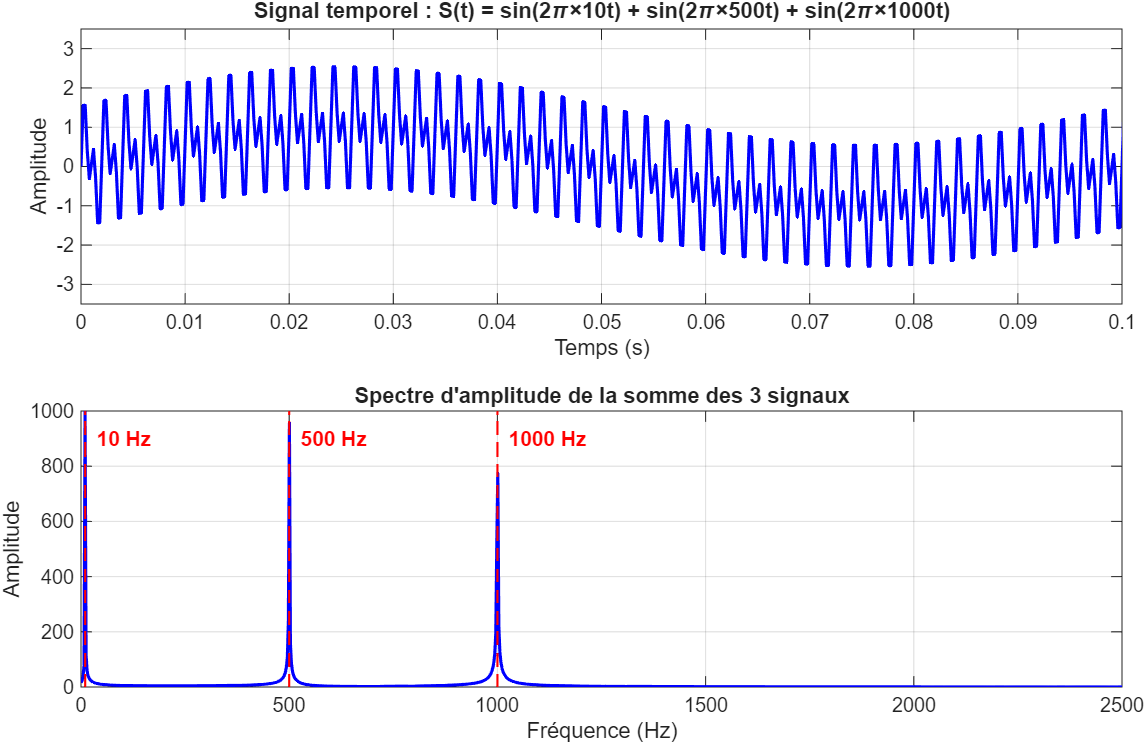
\includegraphics[width=0.8\textwidth]{images/e-1.png}
    \vspace{1cm}}}
    \caption{Signal temporel et spectre de la somme de 3 sinusoïdes (amplitudes égales)}
    \label{fig:somme_amp_egales}
\end{figure}

\subsection{Observations}

\subsubsection{E.1 - Signaux d'amplitude identique (1, 1, 1)}

\begin{itemize}
    \item Le spectre présente 3 pics distincts à 10 Hz, 500 Hz et 1000 Hz
    \item Les 3 pics ont approximativement la même amplitude ($\approx 2500$)
    \item Les pics sont bien séparés et facilement identifiables
    \item Aucune interférence entre les différentes composantes fréquentielles
    \item Le spectre de la somme = somme des spectres individuels (linéarité de la FFT)
\end{itemize}

\subsection{Partie E.b : Signaux d'amplitudes différentes}

\subsubsection{Énoncé}

Même travail en affectant à ces trois signaux les amplitudes respectives suivantes : 10, 1 et 1.

\subsubsection{Signal analysé}

\begin{equation}
    S_2(t) = 10 \sin(2\pi \cdot 10 \cdot t) + \sin(2\pi \cdot 500 \cdot t) + \sin(2\pi \cdot 1000 \cdot t)
\end{equation}

\subsubsection{Paramètres}

Les mêmes paramètres que pour la partie E.a :
\begin{itemize}
    \item $F_s = 5000$ Hz
    \item $N = 2048$ points
\end{itemize}

\begin{figure}[H]
    \centering
    \fbox{\parbox{0.9\textwidth}{\centering\vspace{1cm}
    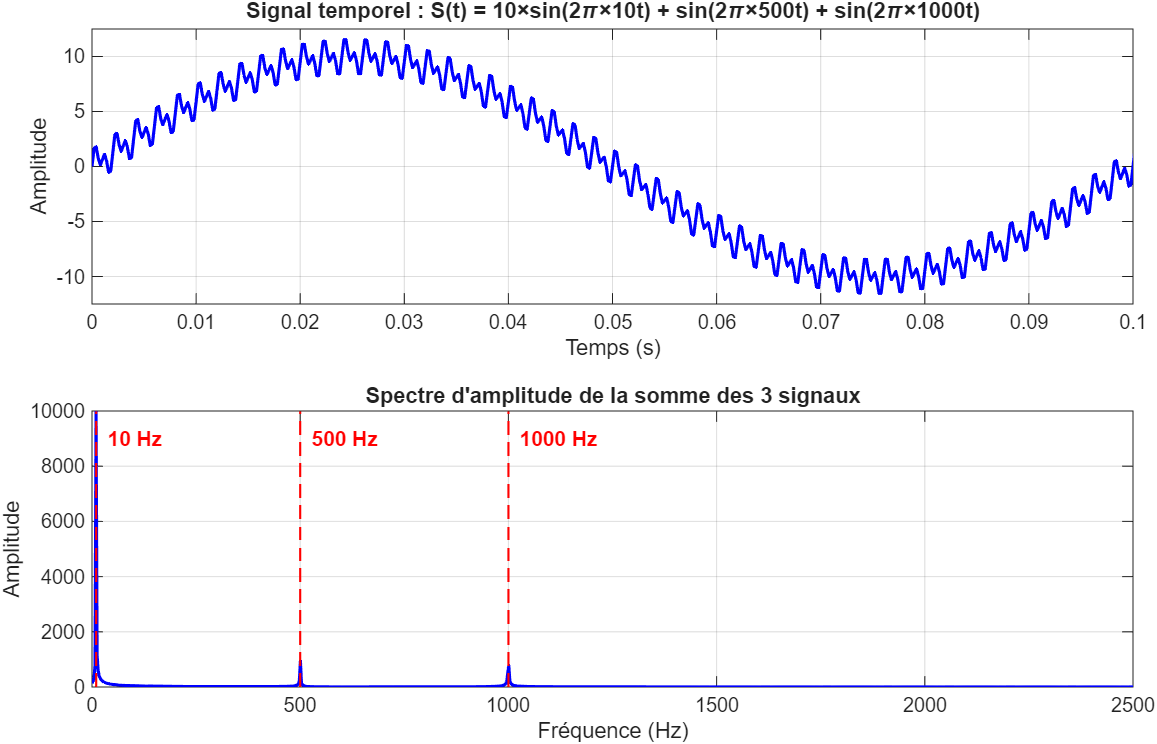
\includegraphics[width=0.8\textwidth]{images/e-2.png}
    \vspace{1cm}}}
    \caption{Signal temporel et spectre de la somme (amplitudes 10, 1, 1)}
    \label{fig:somme_amp_differentes}
\end{figure}

\subsubsection{Observations - E.2 : Signaux d'amplitude différente (10, 1, 1)}

\begin{itemize}
    \item Le spectre présente toujours 3 pics distincts aux mêmes fréquences
    \item Le pic à 10 Hz est beaucoup plus grand ($\approx 25000$) que les autres ($\approx 2500$)
    \item Le rapport d'amplitude entre les pics correspond aux rapports des signaux temporels
    \item Le pic à 10 Hz domine le spectre, reflétant sa plus grande amplitude temporelle
    \item Les pics à 500 Hz et 1000 Hz restent visibles malgré l'écart d'amplitude
\end{itemize}

\subsection{Interprétation des résultats (Parties E.a et E.b)}

\subsubsection{Linéarité de la FFT}

La FFT est une transformation linéaire :

\begin{equation}
    \boxed{\text{FFT}(S_1 + S_2 + S_3) = \text{FFT}(S_1) + \text{FFT}(S_2) + \text{FFT}(S_3)}
\end{equation}

Conséquences :
\begin{itemize}
    \item Le spectre de la somme est la somme des spectres
    \item Chaque composante fréquentielle est préservée
    \item Pas de création de nouvelles fréquences (pas d'intermodulation)
\end{itemize}

\subsubsection{Conservation des amplitudes relatives}

Le rapport des amplitudes spectrales reflète le rapport des amplitudes temporelles :

\begin{equation}
    \text{Si } A_1 = 10 \times A_2, \text{ alors } |\text{FFT}(S_1)| \approx 10 \times |\text{FFT}(S_2)|
\end{equation}

Conséquences :
\begin{itemize}
    \item La FFT préserve l'information d'amplitude
    \item On peut identifier les composantes dominantes du signal
\end{itemize}

\subsubsection{Résolution fréquentielle suffisante}

Avec $\Delta f = 2.44$ Hz, les 3 fréquences sont bien séparées :

\begin{align}
    \text{Écart entre 10 Hz et 500 Hz} &: 490 \text{ Hz} \gg \Delta f \\
    \text{Écart entre 500 Hz et 1000 Hz} &: 500 \text{ Hz} \gg \Delta f
\end{align}

Conséquences :
\begin{itemize}
    \item Les pics ne se chevauchent pas
    \item Identification claire de chaque composante
\end{itemize}

\subsubsection{Importance du choix de $F_s$}

$F_s = 5000$ Hz permet de respecter largement le critère de Shannon :

\begin{equation}
    F_s = 5 \times f_{\max} \gg 2 \times f_{\max} \text{ (Nyquist)}
\end{equation}

Conséquences :
\begin{itemize}
    \item Pas d'aliasing
    \item Représentation fidèle de toutes les composantes
    \item Qualité spectrale excellente
\end{itemize}

\subsection{Conclusion de la partie E}

\subsubsection{Question : Sous quelle condition la FFT permet-elle de constituer et d'observer correctement le spectre d'un signal dont la fréquence maximale est $f$ ?}

Pour constituer et observer correctement le spectre d'un signal de fréquence maximale $f$, les conditions suivantes doivent être respectées :

\textbf{1) CONDITION IMPÉRATIVE - Théorème de Shannon}

\begin{equation}
    \boxed{F_s > 2 \times f \quad \text{(minimum absolu)}}
\end{equation}

\begin{itemize}
    \item C'est la condition MINIMALE obligatoire
    \item Si $F_s \leq 2f$ : aliasing $\rightarrow$ spectre inexploitable et perte irréversible d'information
    \item En pratique : prendre $\boxed{F_s \geq 5 \times f}$ pour une marge de sécurité
\end{itemize}

\textbf{2) Résolution fréquentielle adaptée}

\begin{equation}
    \Delta f = \frac{F_s}{N} \text{ doit être suffisamment petit}
\end{equation}

\begin{itemize}
    \item Si on veut séparer deux fréquences espacées de $\Delta f_{\text{signal}}$, il faut : $\Delta f < \Delta f_{\text{signal}}$
    \item Plus $N$ est grand, meilleure est la résolution
    \item Compromis entre résolution et temps de calcul
\end{itemize}

\textbf{3) Durée d'observation suffisante}

La résolution "réelle" est limitée par :

\begin{equation}
    \Delta f_{\min} = \frac{1}{T_{\text{observation}}}
\end{equation}

\begin{itemize}
    \item Pour observer une fréquence de 10 Hz avec précision, il faut $T \geq 0.1$ s
    \item Dans ce TP : $T = 1$ s permet $\Delta f_{\min} = 1$ Hz
\end{itemize}

\textbf{4) Nombre de points $N$ en puissance de 2}

\begin{itemize}
    \item Optimisation de l'algorithme FFT (complexité $O(N \log N)$)
    \item $N = 128, 256, 512, 1024, 2048, 4096, \ldots$
    \item Calcul plus rapide et efficace
\end{itemize}

\vspace{0.5cm}

\textbf{Synthèse :} Pour un signal de fréquence maximale $f$, il faut impérativement respecter $F_s > 2f$ (Shannon) et choisir un $N$ suffisamment grand pour obtenir une résolution $\Delta f = F_s/N$ permettant de distinguer les composantes fréquentielles d'intérêt.

\newpage

% Conclusion générale
\section{Conclusion générale}

Ce travail pratique sur la génération et l'analyse de signaux avec MATLAB a permis d'explorer de manière approfondie les principes fondamentaux de l'analyse spectrale par FFT (Fast Fourier Transform).

\subsection{Synthèse des enseignements}

\textbf{Le théorème de Shannon} constitue la base incontournable de l'échantillonnage numérique. La condition $F_s > 2f$ est \textbf{impérative} : sa violation entraîne l'aliasing, un phénomène destructeur et irréversible qui rend le spectre inexploitable. Les expérimentations avec différentes fréquences d'échantillonnage ont clairement démontré cette dégradation progressive jusqu'à la disparition complète du pic à $F_s = 200$ Hz.

\textbf{La résolution fréquentielle} $\Delta f = F_s/N$ détermine la finesse de l'analyse spectrale. L'augmentation du nombre de points $N$ améliore la visualisation et permet une meilleure localisation des composantes fréquentielles. Le choix de $N$ doit être un compromis entre précision (N grand) et efficacité de calcul, en privilégiant les puissances de 2 pour optimiser l'algorithme FFT.

\textbf{L'indépendance vis-à-vis du déphasage} a été démontrée : le spectre d'amplitude ne capture que la fréquence et l'amplitude des composantes, ignorant totalement leur phase. Cette propriété est fondamentale pour comprendre les limites de l'analyse spectrale classique.

\textbf{La linéarité de la FFT}, vérifiée à travers l'analyse de signaux composites, confirme que le spectre d'une somme de signaux est la somme des spectres individuels, avec préservation des rapports d'amplitude. Cette propriété est essentielle pour décomposer et analyser des signaux complexes.

\subsection{Réponse à la question centrale}

\textbf{Sous quelle condition la FFT permet-elle de constituer et d'observer correctement le spectre d'un signal dont la fréquence maximale est $f$ ?}

La condition \textbf{absolue et nécessaire} est :

\begin{equation}
    \boxed{F_s > 2 \times f \quad \text{(Théorème de Shannon)}}
\end{equation}

En pratique, on recommande $F_s \geq 5f$ pour garantir une marge de sécurité suffisante.

De plus, il faut choisir un nombre de points $N$ (puissance de 2) permettant d'obtenir une résolution $\Delta f = F_s/N$ adaptée à la séparation des composantes fréquentielles d'intérêt.

\subsection{Perspectives}

Ces concepts fondamentaux constituent un socle pour aborder des techniques plus avancées en traitement du signal :
\begin{itemize}
    \item Filtrage numérique (passe-bas, passe-haut, passe-bande)
    \item Analyse temps-fréquence (transformée de Fourier à court terme, spectrogrammes)
    \item Transformée en ondelettes pour l'analyse de signaux non-stationnaires
    \item Applications pratiques : audio, télécommunications, biomédical, géophysique
\end{itemize}

La maîtrise de la FFT et du théorème de Shannon est indispensable pour tout ingénieur travaillant dans le domaine du traitement du signal numérique.

\end{document}
